%TODO?
\begin{Satz}{Konservativität und Integrabilitätsbedingungen}{}
    Sei $V: (x, y) \mapsto (f_1(x), f_2(y))$ ein Vektorfeld das konservativ ist (= ein Potentialfeld) und $V \in C^1$.
    Dann gelten die \textbf{Integrabilitätsbedingungen}.
    \begin{multicols}{2}
    Für $\R^2$:
    \[ \frac{\partial f_1}{\partial x_2} = \frac{\partial f_2}{\partial x_1} \]
    Für $\R^3$:
    \[ \frac{\partial f_1}{\partial x_2} =  \frac{\partial f_2}{\partial x_1}, 
    ~~  \frac{\partial f_1}{\partial x_3} = \frac{\partial f_3}{\partial x_1},
    ~~ \frac{\partial f_2}{\partial x_3} =  \frac{\partial f_3}{\partial x_2}
    \]
    Für $\R^n$:
    \[
        \frac{\partial f_i}{\partial x_j} =  \frac{\partial f_j}{\partial x_i},
        \quad
        \forall i \neq j,
        \quad
        i, j \in \{1,...,n\}
    \]
    \end{multicols}
\end{Satz}

\begin{Definition}{Sternförmig}{}
    Eine Menge $X$ ist sternförmig, wenn es ein $x_0 \in X$ gibt, so dass für $x \in X$ gilt, dass das Linienstück das $x_0$ und $x$ verbindet in $X$ ist. 
    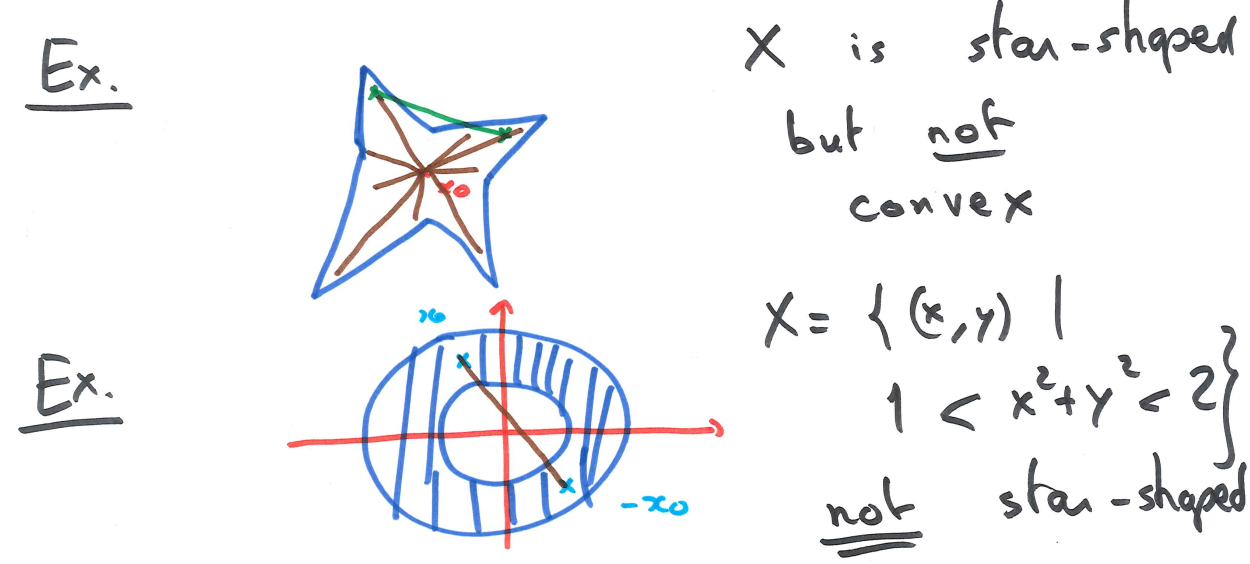
\includegraphics[width = 18em]{starshape}
\end{Definition}

\begin{Satz}{Sternförmig}{}
    Sei $X$ sternförmig und offen. Und $f$ ein $C^1$ Vektorfeld. Und 
    \[\frac{\partial f_i}{\partial x_j}=\frac{\partial f_j}{\partial x_i}\] auf X für alle $i \neq j$.
    Dann ist $f$ konservativ.

\end{Satz}

\begin{Definition}{Curl oder Rotation eines Vektorfeldes}{}
    Sie $X\subset \mathbb{R}^3$ und $f:X \rightarrow \mathbb{R}^3$ ein $C^1$ Vektorfeld.
    \[   
        \text{curl}(f) =
        \left(
        \begin{array}{c}
        \partial_{y}f_3 - \partial_zf_2\\
        \partial_zf_1 - \partial_x f_3\\
        \partial_xf2-\partial_yf_1\\
        \end{array}
        \right)
    \]
    Oder mittelhilfe det Determinante
    \[
        \text{curl}(f)=
        \begin{vmatrix}
        e_1 & e_2 & e_3\\
        \partial_x & \partial_y & \partial_z \\
        f_1 & f_2 & f_3\\
        \end{vmatrix}
    \]
\end{Definition}